%\usepackage{xcite}
%\externalcitedocument{bibliography}
	\chapter{Quantum Walks}
	   % Falar dos varios tipos de caminhada quantica sem circuito \\
	   % talvez simulaçoes em python?? \\
    %     ambainis2004 - Pasta introqw/Coin\\
    %     introducao com random walks classicas\\
    %     Meter resultados simulaçoes de python.
            \textcolor{red}{Precisamos fazer uma introdução aqui, descrever o conteúdo do capítulo, algumas referências se necessário. Não precisa ser muito longo.}
	    \input{Chapters/Chapter3/Sections/CoinedQuantumWalk}
	        	\section{Continuous-Time Quantum Walk}\label{contwalk}
    	        The continuous-time random walk model on a graph is a Markov process where transitions have a fixed probability per unit time $\gamma$ of moving to adjacent vertices, firstly introduced by \cite{montrollweiss1965}. Consider a graph $G$ with $N$ vertices and no self-loops, this walk can be defined by the linear differential equation that describes the probability of jumping to a connected vertex in any given time \textcolor{red}{pode colocar G(V,E) e depois especificar que (i,j) é uma aresta}
    	        \begin{equation}
    	            \frac{dp_i(t)}{dt} = \gamma \sum_j L_{ij} p_j(t), \label{contWalk}
    	        \end{equation}
    	        where $L$ is the Laplacian defined as $L = A - D$. $A$ is the adjacency matrix that represents each vertex connection, given by
    	        \begin{equation}
    	           A_{ij} = \begin{cases} 1, & \mbox{if } (i,j)\in G \\ 0, & \mbox{otherwise,} \end{cases}
    	        \end{equation}
    	        and D is the diagonal matrix $D_{jj} = deg(j)$ corresponding to the degree\footnote{The degree of a vertex refers to the number of edges that it is connected to.} of a vertex $j$.
    	        
                In the quantum case, the nodes are quantum states that form the basis for the Hilbert space. The continuous-time quantum walk model will also be described by a differential equation, the Schrödinger equation
                \begin{equation}
                    i\hbar \frac{d\ket{\Psi(t)}}{dt} = \hat{H} \ket{\Psi(t)}, \label{shrodinger}
                \end{equation}
                where $\hat{H} = -\gamma L$ is the Hamiltonian of the system. More explicitly,
                \begin{equation}
                    \hat{H}_{ij} = \begin{cases} 
                            deg(j)\gamma, & \mbox{if } i= j; \\ 
                            -\gamma, & \mbox{if } i\neq j\mbox{ and adjacent};\\
                            0, & \mbox{if } i\neq j\mbox{ and not adjacent}.
                        \end{cases}.
                        \label{Hamilt}
                \end{equation}\par
                A general state of a system $\ket{\Psi(t)}$ can be written as a function of it's complex amplitudes \textcolor{red}{acredito que seja contrária a relação, as amplitudes que são descritas pelo estado através da equação 28}
                \begin{equation}
                    q_i = \braket{i|\Psi(t)},
                \end{equation}
                which means \ref{shrodinger} can be rewritten as 
                \begin{equation}
                     i\hbar \frac{dq_i(t)}{dt} = \sum_j \hat{H}_{ij} q_j(t).
                \end{equation}
                This highlights the similarities between the Schrödinger equation and \ref{contWalk}. One of the main differences is the complex phase $i$, which will result in a very different behaviour. \textcolor{red}{você pode dizer que a 29 é uma quantização da 24}\par
                Setting $\hbar = 1$ and solving the differential equation results in the evolution operator of this walk \textcolor{red}{acho que podemos ajustar, talvez a equação 32 deva subir, porque ela que é solução da equação diferencial}%mencionar redimens. devido ao planck modificado
            	\begin{equation}
            	    U(t) = e^{-iHt} = e^{i(-\gamma L)t} = e^{-i\gamma(A+D)t}
            	\end{equation}
            	In the regular graph case, where $D$ is simply the degree of the whole graph multiplied by the identity matrix, $A$ and $D$ will commute, meaning that the evolution operator can be written in terms of the adjacency matrix \textcolor{red}{ficou muito bom isso daqui}
            	\begin{equation}
            	   U(t) = e^{-i\gamma A t + i\gamma D t} = e^{-i\gamma A t} e^{i\gamma D t} = \phi(t) e^{-i\gamma A t} 
            	\end{equation}
            	since the degree matrix becomes a global phase.
            	%that can be verified by expanding the %exponential function in Taylor series.
            	%Demonstrar com eq dif ordinarias de variaveis separaveis.
            	Applying this operator to an initial condition $\Psi(0)$, will give the state of the system at a time $t$
                \begin{equation}
                    \ket{\Psi(t)} = U(t)\ket{\Psi(0)}.
                \end{equation}\par
                Considering a uni-dimensional quantum system, each vertex will have at most 2 other neighboring vertices, reducing equation \ref{Hamilt} to
                \begin{equation}
                \hat{H}_{ij} = \begin{cases} 
                            2\gamma, & \mbox{if } i= j; \\ 
                            -\gamma, & \mbox{if } i\neq j\mbox{ and adjacent};\\
                            0, & \mbox{if } i\neq j\mbox{ and not adjacent}.
                        \end{cases}
                \end{equation}\par
                For a more detailed visualization, this quantum walk model was coded in python and figure \ref{fig:contdist0} was obtained setting the transition rate to $\gamma=\frac{1}{2\sqrt{2}}$ the initial condition to $\ket{\Psi(0)} = \ket{0}$ \textcolor{red}{cortou a figura}
                
                \begin{figure}[!h]
                    \centering
                    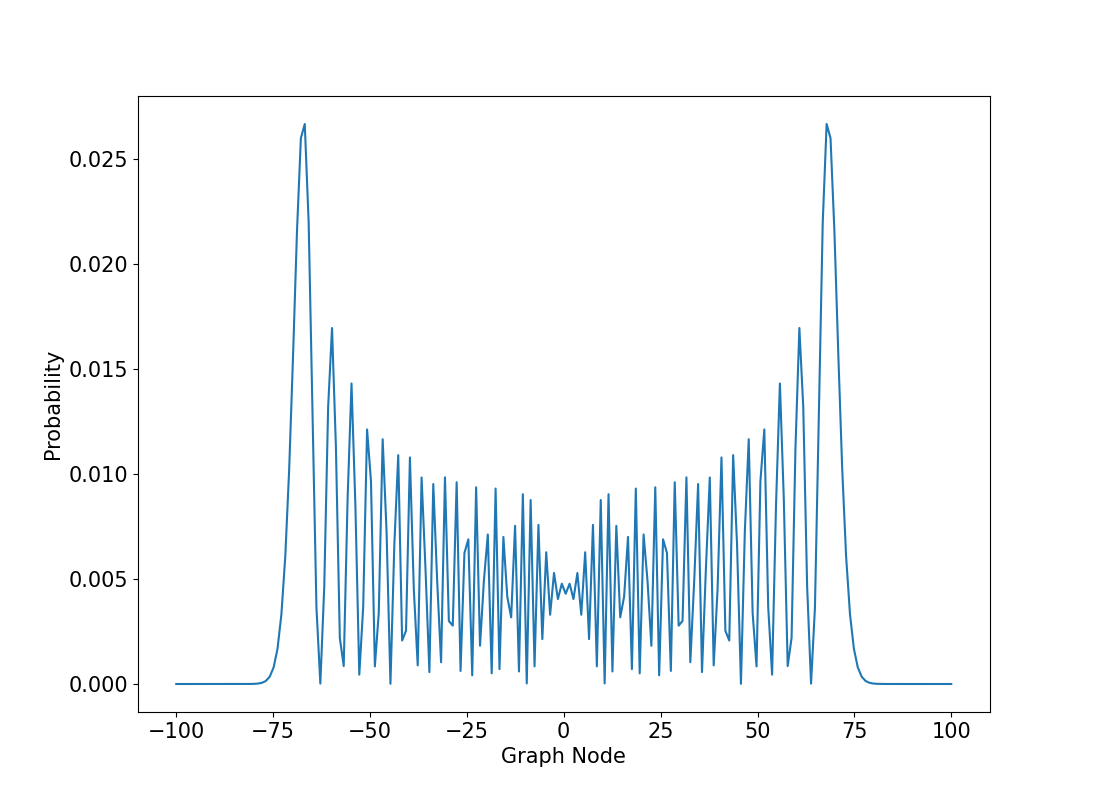
\includegraphics[scale=0.40]{img/ContQuantumWalk/ctqwSinglePsi0.png}
                    \caption{Probability distribution for the continuous-time quantum walk on a line, at t = 100, with initial condition $\ket{\Psi(0)}=\ket{0}$ and $\gamma=\frac{1}{2\sqrt{2}}$.} 
                    \label{fig:contdist0}
                \end{figure}
                
            A brief look at figure \ref{fig:contdist0} reveals several similarities to the coined quantum walk model of figure \ref{fig:coinedwalk3}. Both have two peaks away from the origin and low probability near the origin.
             However, in the previous quantum walk, these characteristics were altered as a function of the chosen coin and initial condition, whereas in this case different values of $\gamma$ will influence the probability distribution. For example, a lower value of $\gamma$ will limit the spread of the probability distribution, as is shown in figure \ref{fig:contdist1}. \textcolor{red}{você pode dizer que o desvio padrão é proporcional ao $\gamma$ também}
                \begin{figure}[!h]
                    \centering
                    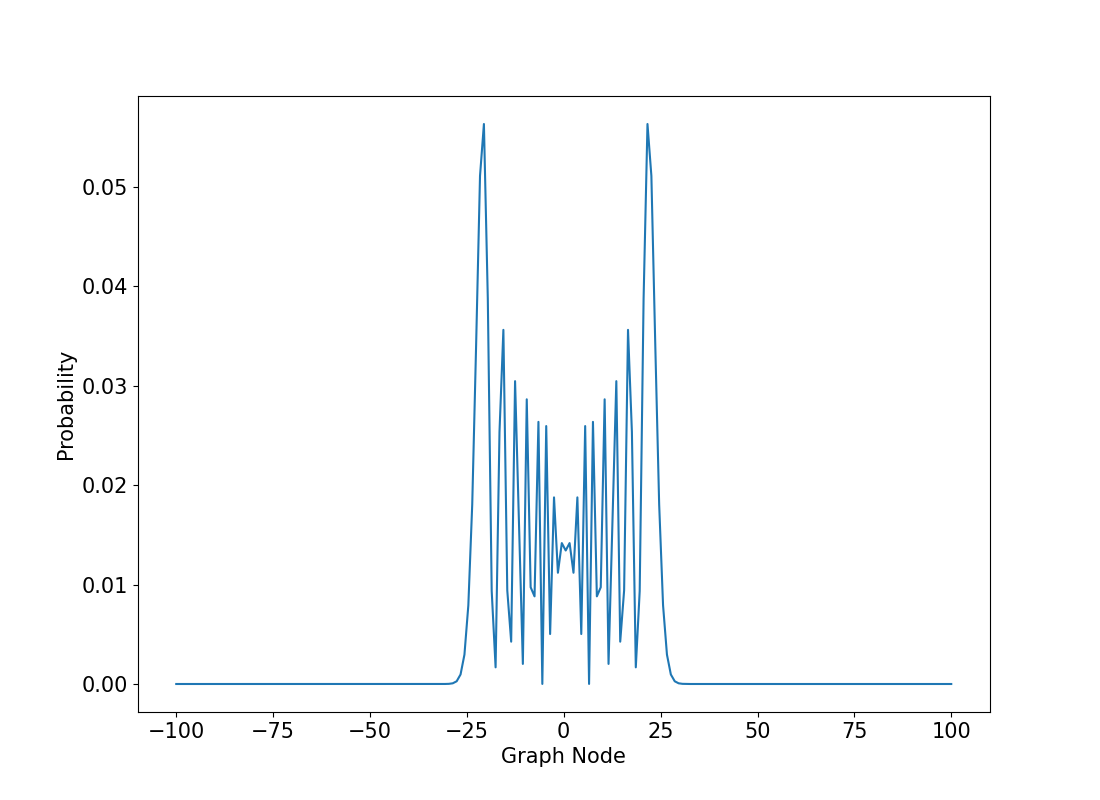
\includegraphics[scale=0.40]{img/ContQuantumWalk/ctqwSinglePsi0LowerGamma.png}
                    \caption{Probability distribution for the continuous-time quantum walk on a line, after 100 steps, with initial condition $\ket{\Psi(0)}=\ket{0}$ and $\gamma=\frac{1}{6\sqrt{2}}$.} 
                    \label{fig:contdist1}
                \end{figure}
                
                \begin{figure}[!h]
                    \centering
                    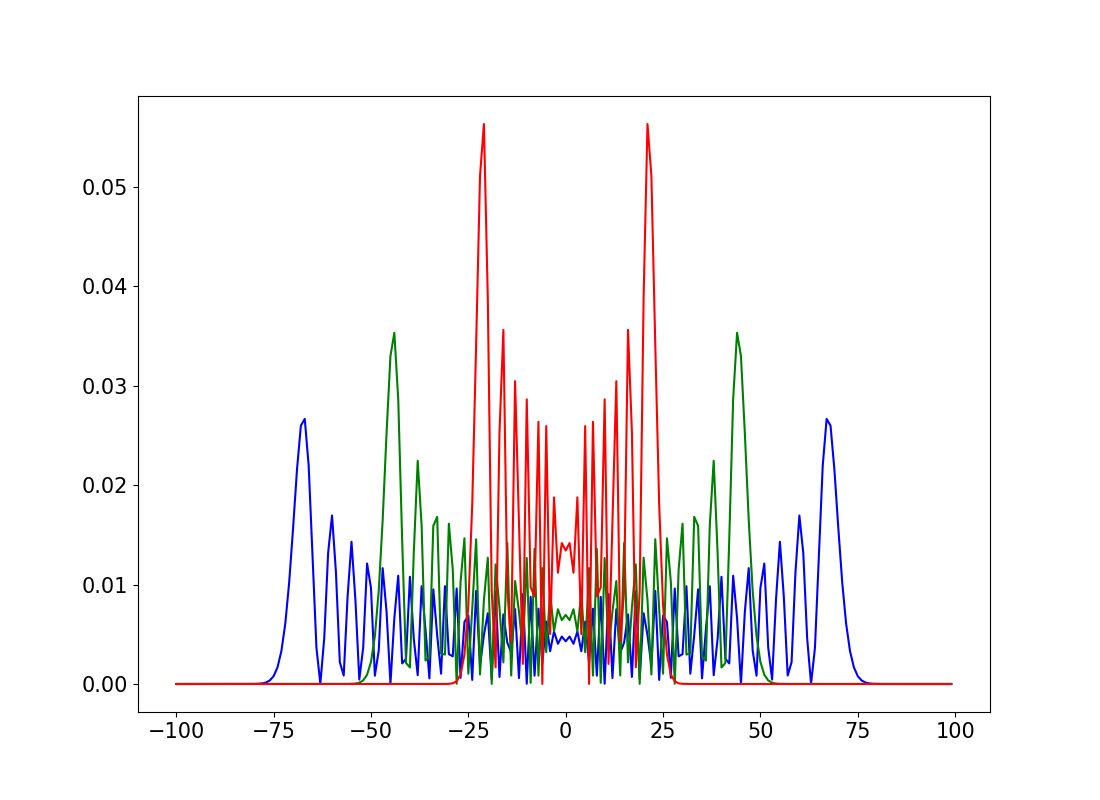
\includegraphics[scale=0.40]{img/ContQuantumWalk/ctqwMultipleGamma.png}
                    \caption{Temporary} 
                    \label{fig:contdist1}
                \end{figure}
                
            Moreover, the effects of altering the initial condition will also differ in the continuous-time example. For example, setting the initial condition to the balanced superposition of states $\ket{0}$ and $\ket{1}$ has no effect on the overall pattern of the probability distribution as can be seen in figure \ref{fig:contdist2}. Both peaks still are still present and at the same distance from the origin, with intermediate amplitudes being attenuated relative to figure \ref{fig:contdist0}. This behaviour is in contrast with the discrete-time case, where a change in the initial condition would dictate the number of peaks and where they would appear.
            
                \begin{figure}[!h]
                    \centering
                    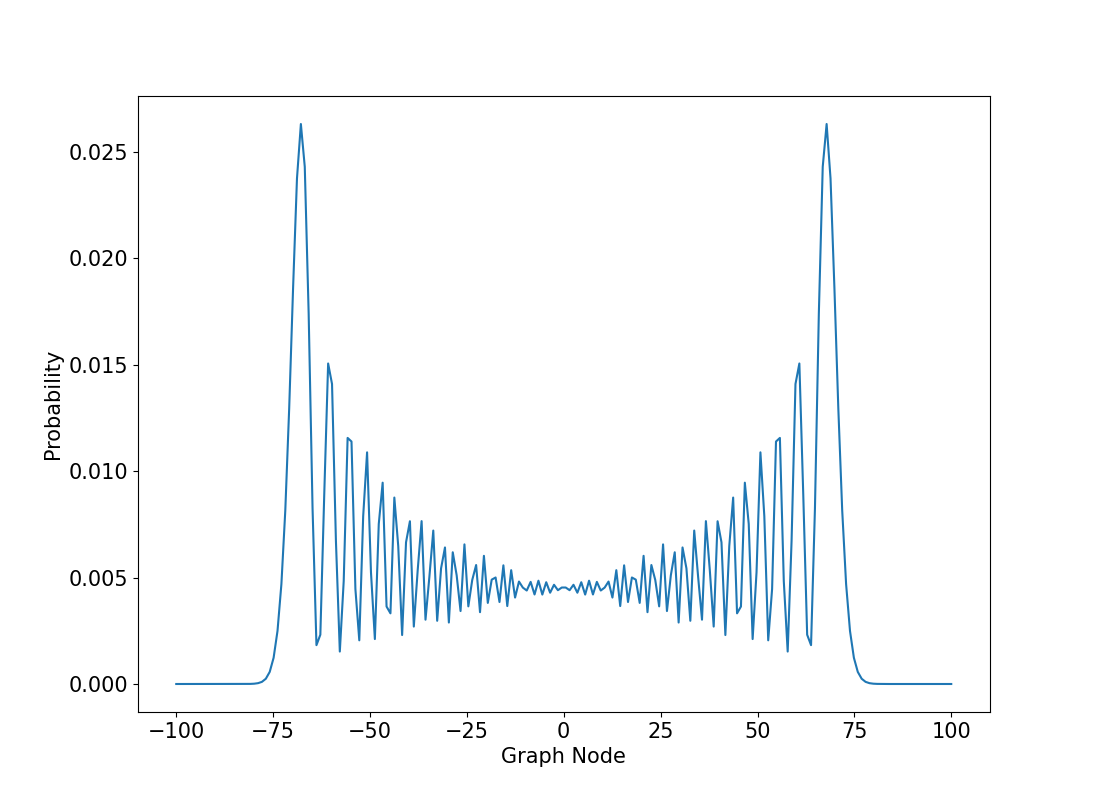
\includegraphics[scale=0.40]{img/ContQuantumWalk/ctqwSingleSup.png}
                    \caption{Probability distribution for the continuous-time quantum walk on a line, after 100 steps, with initial condition $\ket{\Psi(0)}=\frac{\ket{0}+\ket{1}}{\sqrt{2}}$ and $\gamma=\frac{1}{2\sqrt{2}}$.} 
                    \label{fig:contdist2}
                \end{figure}
                
                \begin{figure}[!h]
                    \centering
                    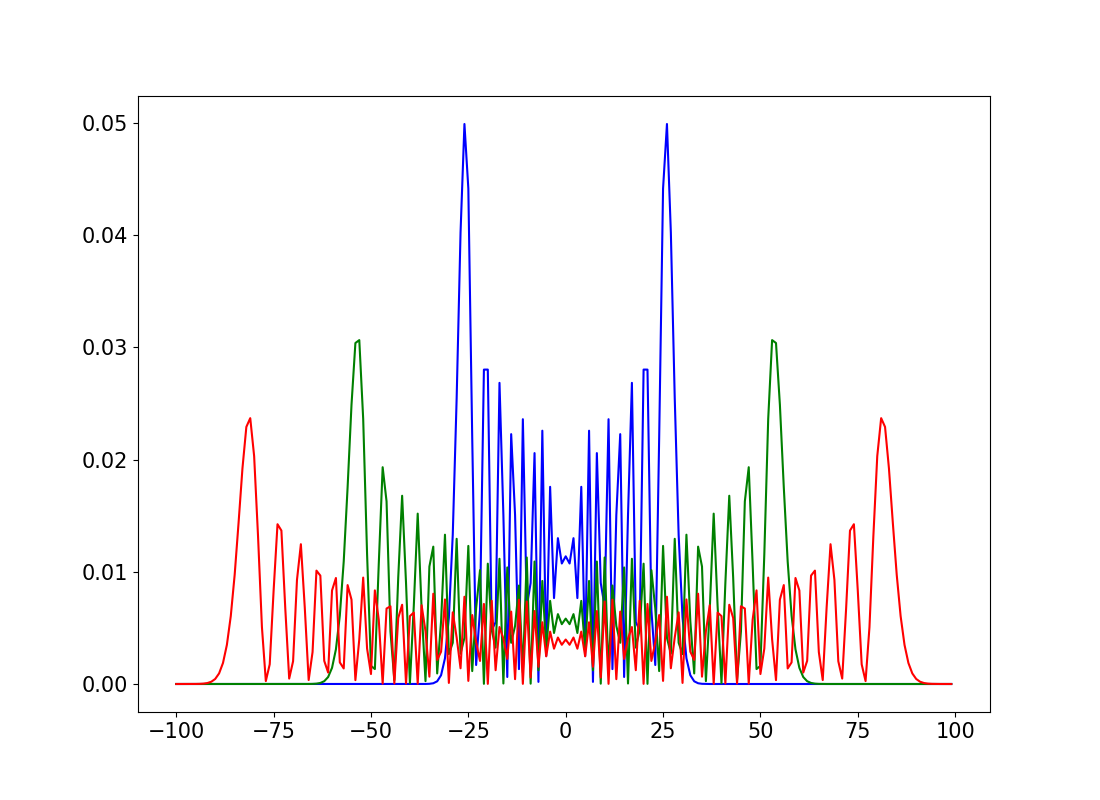
\includegraphics[scale=0.40]{img/ContQuantumWalk/ctqwMultipleTime.png}
                    \caption{Temporary} 
                    \label{fig:contdist2}
                \end{figure}
                
             \textcolor{red}{precisa de um fechamento aqui também, alguns resultdos e referências mais talvez}
             
                \clearpage
                

	                \section{Staggered Quantum Walk}\label{stagWalk}
            	Similarly to the continuous-time quantum walk, the staggered case aims to spread a transition probability to neighboring vertices but with discrete time steps. The notion of adjacency now comes from cliques\footnote{A clique is defined as the subset of vertices of an undirected graph such that every two distinct vertices in each clique are adjacent.}, and the initial stage of this walk consists in partitioning the graph in several different cliques. This is called tessellation, and it is defined as the division of the set of vertices into disjoint cliques. An element of a tessellation $\mathscr{T}$ is called a polygon, and it's only valid if if all of its vertices belong to the clique in $\mathscr{T}$. The set of polygons of each tessellation must cover all vertices of the graph, and the set of tessellations ($\mathscr{T}_{1}$,$\mathscr{T}_{2}$,...,$\mathscr{T}_{k}$) must cover all edges.\par
            	These definitions allow the construction of operators $H_1$,$H_2$,...,$H_k$ that will be used to propagate the probability amplitude locally, in each polygon. The state associated to each polygon is
            	\begin{equation}
            	    \ket{u_{j}^{k}} = \frac{1}{\sqrt{\mathopen|\alpha_{j}^{k}}\mathclose|}\sum_{l\in\alpha_{j}^{k}}\ket{l}
            	\end{equation}
            	where $\alpha_{j}^{k}$ is the $j-th$ polygon in the $k-th$ tessellation.\par
            	The unitary and Hermitian operator $H_k$, associated to each tessellation is defined in \cite{portugal2017b} as
            	\begin{equation}
            	    H_k = 2\sum_{j=1}^{p}\ket{u_{j}^{k}}\bra{u_{j}^{k}} - I
            	    \label{eq:StagHamil}
            	\end{equation}\par
            	Solving the time-independent Schrodinger equation for this Hamiltonian gives the evolution operator
            	\begin{equation}
            	    U = e^{i\theta_{k}H_{k}}...e^{i\theta_{2}H_{2}}e^{i\theta_{1}H_{1}}
            	    \label{eq:stagWalkUnmodOp}
            	\end{equation}
            	where
            	\begin{equation}
            	    e^{i\theta_{k}H_{k}} = \cos{(\theta_k)}I + i\sin{(\theta_k)}H_k
            	\end{equation}
            	since $H_k^2 = I$.\textcolor{red}{trocar and por since. Posso referir livro do nielsen}\par
            	The simplest use case of this quantum walk model is the one-dimensional lattice, where the minimum tessalations are
            	\begin{equation}
            	    \mathscr{T}_{\alpha}= \{\{2x,2x+1\}\colon x \in \Z\}
            	\end{equation}
            	\begin{equation}
            	    \mathscr{T}_{\beta}= \{\{2x+1,2x+2\}\colon x \in \Z\}
            	\end{equation}
            	 Each element of the tessellation has a corresponding state, and the uniform superposition of these states is
            	\begin{equation}
            	    \ket{\alpha_x} = \frac{\ket{2x} + \ket{2x+1}}{\sqrt{2}}
            	\end{equation}
            	\begin{equation}
            	    \ket{\beta_x} = \frac{\ket{2x+1}+\ket{2x+2}}{\sqrt{2}}
            	\end{equation}\par
            	One can now define Hamiltonians $H_\alpha$ and $H_\beta$ as \textcolor{red}{trocar operators por hamiltonians, talvez} 
            	\begin{equation}
            	    H_\alpha = 2\sum_{x=-\infty}^{+\infty}\ket{\alpha_{x}}\bra{\alpha_x} - I
            	\end{equation}
            	\begin{equation}
            	    H_\beta = 2\sum_{x=-\infty}^{+\infty}\ket{\beta_{x}}\bra{\beta_x} - I
            	\end{equation}\par
            	The Hamiltonian evolution operator reduces to
            	\begin{equation}
            	    U = e^{i\theta H_\beta}e^{i\theta H_\alpha}
            	\end{equation}
                and applying it to an initial condition $\ket{\Psi(0)}$ results in the time evolution operator
                \begin{equation}
                    U\ket{\Psi(t)} = U^t\ket{\Psi(0)}
                \end{equation}\par
                Having defined the time evolution operator, the walk is ready to be coded with a certain initial condition and $\theta$ value, to better understand how the probability distribution spreads through time. \textcolor{red}{você pode acrescentar que o $\theta$ terá um papel similar ao $\gamma$ no controle do desvio-padrão}
                
                For the first case study, the initial condition will be a uniform superposition of states $\ket{0}$ and $\ket{1}$ and the $\theta$ value will be varied in order to understand how this parameter impacts the walk
                
            	\begin{figure}[!h]
                    \centering
                    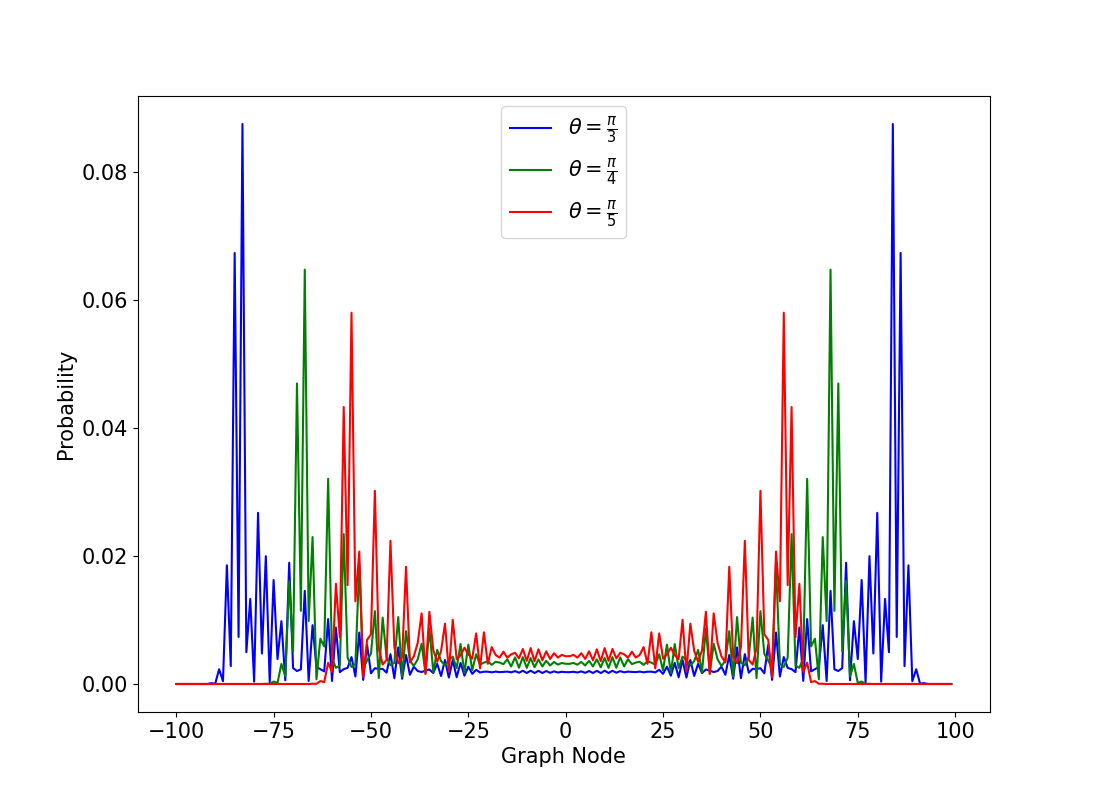
\includegraphics[scale=0.40]{img/StagQuantumWalk/stagqwMultiple.png}
                    \caption{Probability distribution for the staggered quantum walk on a line after 50 steps, with initial condition $\ket{\Psi(0)}=\frac{\ket{0}+\ket{1}}{\sqrt{2}}$, for multiple angles.} 
                    \label{fig:fig5}
                \end{figure}
                
                The overall structure of the probability distribution remains the same, the difference is that the walker is more likely to be found further away from the origin as the angle increases.\par
                Another interesting case study is to see how the initial condition affects the dynamics of the system
                
                \begin{figure}[!h]
                    \minipage{0.55\textwidth}
                        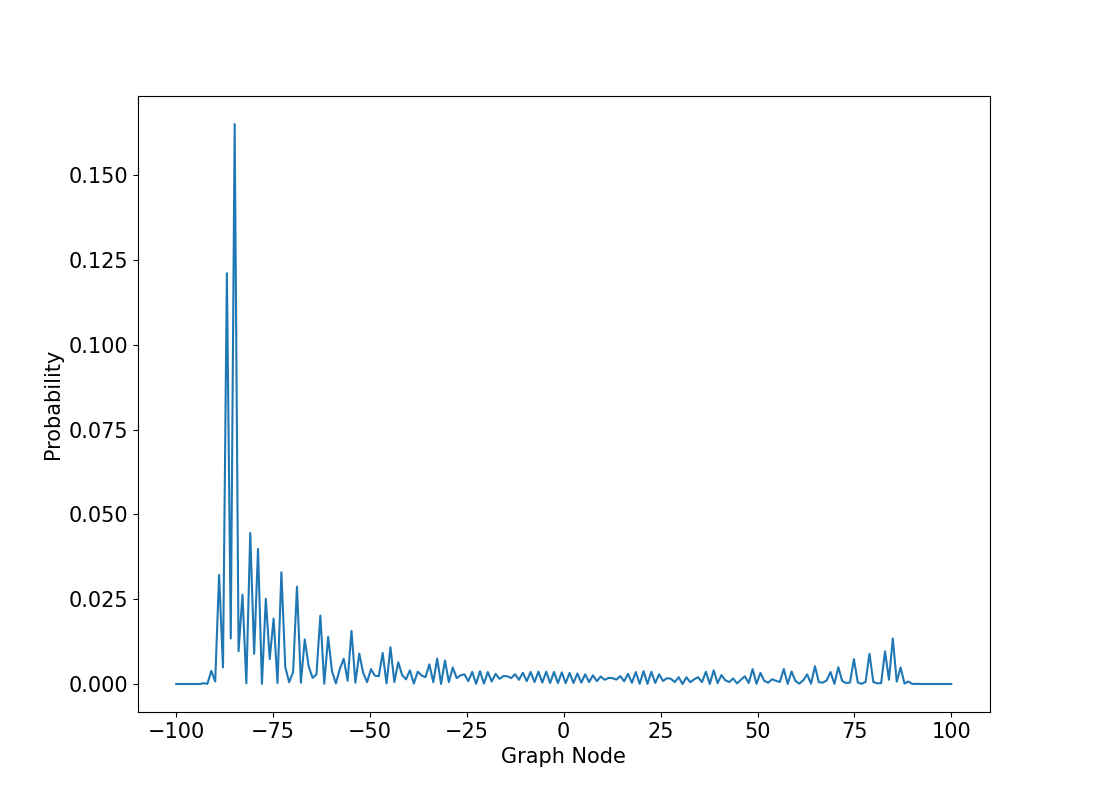
\includegraphics[width=\linewidth]{img/StagQuantumWalk/stagqwSingle0.png}
                        \caption{$\ket{\Psi(0)}=\ket{0}$}\label{fig:fig6}
                    \endminipage\hfill
                        \minipage{0.55\textwidth}
                        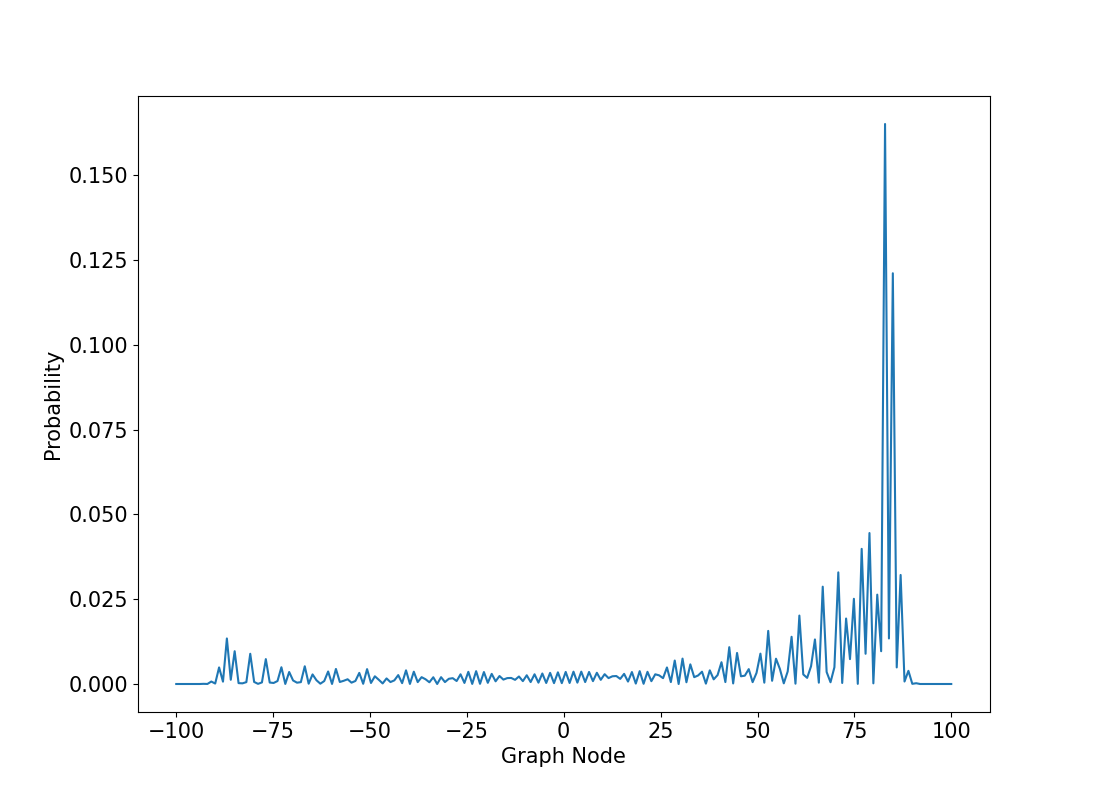
\includegraphics[width=\linewidth]{img/StagQuantumWalk/stagqwSingle1.png}
                      \caption{$\ket{\Psi(0)}=\ket{1}$}\label{fig:fig7}
                    \endminipage\hfill
                \end{figure}
                
                Similarly to the coined case, each initial condition results in asymmetric probability distributions, $\ket{\Psi(0)}=\ket{0}$ leads to a peak  in the left-hand side while condition $\ket{\Psi(0)}=\ket{1}$ results in a peak in the right-hand side. As was shown in \ref{fig:fig5}, the uniform superposition of both these conditions results in a symmetric probability distribution.
                 \textcolor{red}{acho que você pode explicar um pouco mais o papel de $\theta$ através dos gráficos e podemos pensar se fazemos gráficos do desvio-padrão para este e o contínuo}

	            \section{Search problems with Quantum Walks}
               In classical computation, a \textit{spatial search problem} focuses on finding marked points in a finite region of space. Defining this region with graphs is fairly straightforward, the vertices of the graph are the search space, and the edges define what transitions are possible through the search space. As was previously mentioned in \ref{chapGrover}, exhaustively searching through an unstructured space, by means of a classical random walk for example, would mean that in the worst case, one would have to take as many steps to find the marked points as there are vertices in the graph. Quantum computing provides an alternative to this complexity through Grover's algorithm, and applying some of his ideas to the coined quantum walk not only allows a quantum counterpart to the random walk search, but also further insight into the algorithm itself.\par
                \textcolor{red}{acho que você precisa delimitar o que fará ao longo desta seção, dizer que tratará os três modelos e a busca}
        \subsection{Coined}
                Following \cite{REN1}'s definition, a good first step is to borrow the diffusion from Grover's algorithm and invert the sign of the state corresponding to the marked vertex while leaving unmarked vertices unchanged. This is done through the following operator \textcolor{red}{eu trocaria a notação de $\mathcal{F}$ por $\mathcal{O}$ e dizer que é um oráculo}
                \begin{equation}
                    \mathcal{F'} = I - 2 \sum_{x\in M} \ket{x}\bra{x}
                \end{equation}
                where M is the set of marked vertices and $\mathcal{F'}$ is an analogue to Grover's oracle. For one marked vertex, this oracle can be written as \textcolor{red}{você pode até dizer que $M=\{0\}$}
                \begin{equation}
                    \mathcal{F'} = I - 2 \ket{0}\bra{0}
                \end{equation}
                Notice that there is no loss of generality by choosing the marked vertex as $0$, since the labelling of the vertices is arbitrary.\par
                The next step is to combine the evolution operator from the coined quantum walk model with the oracle
                \begin{equation}
                    U'= U\mathcal{F'}
                    \label{eq:43}
                \end{equation}
                Similarly to the simple coined case, the walker starts at $\ket{\Psi(0)}$ and evolves following the rules of an unitary operator $U$ followed by the sign inversion of marked vertices. The walker's state after an arbitrary number of steps will be
                \begin{equation}
                    \Psi(t) = (U')^t\ket{\Psi(0)}.
                    \label{eq:sysStateSearch}
                \end{equation}\par
    
                For a better understanding of the search problem in the coined quantum walk model, consider a graph where all the vertices are connected and each vertex has a loop that allows transitions to itself, as shown in figure \ref{fig:undCompGraph}. \textcolor{red}{não precisa dizer que são arcos também}
%                \begin{figure}[!h]
%                \centering
%                \begin{tikzpicture}[shorten >=1pt,auto,node distance=3cm,
%                    thick,main node/.style={circle,draw,font=\sffamily\Large\bfseries}]
%
%                      \node[main node] (1) {1};
%                      \node[main node] (2) [below left of=1] {2};
%                      \node[main node] (3) [below right of=2] {3};
%                      \node[main node] (4) [below right of=1] {4};
%                    
%                      \path[every node/.style={font=\sffamily\small}]
%                        (1) edge node [left] {} (4)
%                            edge [loop above] node {} (1)
%                            edge node [below] {} (3)
%                        (2) edge node [right] {} (1)
%                            edge node {} (4)
%                            edge [loop left] node {} (2)
%                        (3) edge node [right] {} (2)
%                            edge [loop below] node {} (3)
%                        (4) edge node [left] {} (3)
%                            edge [loop right] node {} (4)
%                 \end{tikzpicture}
%                  \caption{Undirected Complete Graph}
%                  \label{fig:undCompGraph}
%                \end{figure}
%                \textcolor{red}{acho que não há necessidade das figuras e dizer que é com grafo direcionado}
%                Grover's algorithm is equivalent to a coined quantum walk on a directed complete graph with loops such as the one in figure \ref{fig:dirCompGraph}.
%                \begin{figure}[!h]
%                    \centering
%                    \begin{tikzpicture}[->,>=stealth',shorten >=1pt,auto,node distance=3cm,
%                    thick,main node/.style={circle,draw,font=\sffamily\Large\bfseries}]
%                      \node[main node] (1) {1};
%                      \node[main node] (2) [below left of=1] {2};
%                      \node[main node] (3) [below right of=2] {3};
%                      \node[main node] (4) [below right of=1] {4};
%                      \path[every node/.style={font=\sffamily\small}]
%                        (1) edge node [bend left] {} (4)
%                            edge [bend right] node[left] {} (2)
%                            edge [loop above] node {} (1)
%                            edge node [arc below] {} (3)
%                        (2) edge node [bend right] {} (1)
%                            edge node {} (4)
%                            edge [loop left] node {} (2)
%                            edge [bend right] node[left] {} (3)
%                        (3) edge node [right] {} (2)
%                            edge [bend right] node[right] {} (4)
%                            edge node [bend up] {} (1)
%                        (4) edge node [left] {} (3)
%                            edge [loop right] node {} (4)
%                            edge [bend right] node[right] {} (1)
%                            edge node [bend left] {} (2);
%                    \end{tikzpicture}
%                    \caption{Directed complete graph with N=4 nodes.}
%                    \label{fig:dirCompGraph}
%                \end{figure}    
%                
                The next step is to label the arcs using notation $\{(v,v'), v \geqslant 0 \land v' \leqslant N-1\}$ 
                where $N$ is the total number of vertices and $(v,v')$ are the position and coin value, respectively, in the coined model. 
                %sera que vale a pena desenhar um grafo com labels?
                The shift operator, now called \texit{flip-flop} shift operator, is
                \begin{equation}
                    S\ket{v1}\ket{v2} = \ket{v2}\ket{v1}.
                \end{equation}\par
                The coin operator is defined as
                \begin{equation}
                    C = I_N \otimes G
                \end{equation}
                where \textcolor{red}{prefiro s a D}
                \begin{equation}
                    G = 2\ket{D}\bra{D} - I
                \end{equation}
                is the Grover coin with $\ket{D}$ being the diagonal state of the coin space. Given both of these operators, the evolution is defined for the unmarked case similarly to \ref{coinedUnmarkedOperator}
                \begin{equation}
                    U = S(I \otimes G).
                \end{equation}\par
                Marking an element in a complete graph is done through the following oracle
                \begin{equation}
                    \mathcal{F''} =\mathcal{F'}\otimes I = (I_N - 2\ket{0}\bra{0})\otimes I_N = I_{N^2} - 2 \sum_v \ket{0}\ket{v}\bra{0}\bra{v} ,
                \end{equation}
                that can be seen, in the arc notation, as an operator that marks all arcs leaving $0$.\par
                Recalling \ref{eq:43}, the modified evolution operator can be written as
                \begin{equation}
                    U' = S(I \otimes G)\mathcal{F''} = S(I \otimes G)\mathcal{F'} \otimes I = S (\mathcal{F'} \otimes G),\label{modifiedEvoCoined}
                \end{equation}
                and the state of the system will evolve according to equation \ref{eq:sysStateSearch}.\par
                As was shown in \cite{REN1}, maximum probability of the marked vertex is achieved after $\frac{\pi}{2}\sqrt{N}$ steps. Figure \ref{fig:coinedSearch} is the result of coding and plotting the evolution of this probability distribution, for graphs of varying sizes. It shows that the probability is close to one at \textit{approximately} the predicted ideal steps, because of the discrete nature of the walk. The probability distributions have a stair-like shape, because transitions in this model only occur on even numbered time steps, because of how the unmodified evolution operator was constructed.
                
            	\begin{figure}[!h]
                    \centering
                    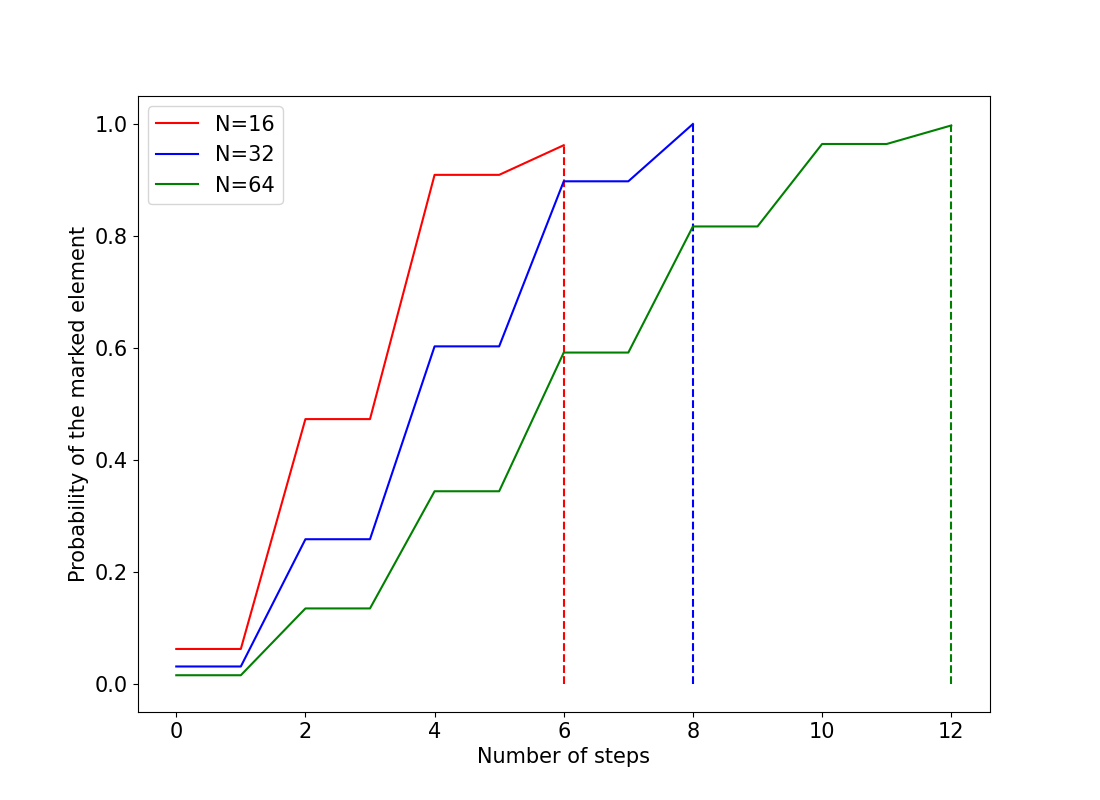
\includegraphics[scale=0.40]{img/CoinedQuantumWalk/Search/CoinedSearch163264.png}
                     \caption{Discrete-time coined quantum walk search for a complete graph with 16, 32 and 64 nodes.}\label{fig:coinedSearch}
                \end{figure}
                
               \subsection{Staggered}
               The process for defining the search problem in this model is similar to the coined quantum walk case. The oracle still inverts the sign of a certain state and amplifies it, and the system's state will still be described by equation \ref{eq:sysStateSearch}. However,instead of using a coin, the staggered model takes advantage of the notions of cliques and tessellations, as was shown in chapter \ref{stagWalk}, which means the unmodified evolution operator has to be defined for an undirected complete graph.\par
               As was shown in figure \ref{fig:undCompGraph}, the vertices in a complete graph are all neighbors. This is a special case because this is the only connected graph where the tessellation cover can be done by one tessellation, since the graph is it's own clique. The minimum tessellations required to cover this structures are defined by the one clique that encompasses all $N$ nodes of the graph
               \begin{equation}
                   \mathscr{T}_{\alpha} = \{\{0,1,2,...,N-1\}\}.
               \end{equation}\par
               The associated polygon can then be described as the balanced superposition of all the nodes in the graph
               \begin{equation}
                   \ket{\alpha} = \frac{1}{\sqrt{N}} \sum_{v=0}^{N-1} \ket{v}.
               \end{equation}\par
               The Hamiltonian, as defined in \ref{eq:StagHamil}, is \textcolor{red}{falta índice no somatório}
               \begin{equation}
                   H_\alpha = 2\sum_0^1\ket{\alpha}\bra{\alpha} - I = 2\ket{\alpha_0}\bra{\alpha_0} - I
               \end{equation}\par
               The unmodified evolution operator from equation \ref{eq:stagWalkUnmodOp}
               \begin{equation}
                   	U = e^{i\theta_{k}H_{k}}...e^{i\theta_{2}H_{2}}e^{i\theta_{1}H_{1}}
               \end{equation}
               reduces to the single Hamiltonian case
               \begin{equation}
                   U = e^{i\theta H_\alpha}.
                   \label{eq:stagQWSearchUnmodEvo1}
               \end{equation}\par
               The choice of the $\theta$ value is an important one, since maximum probability is achieved at $\theta = \frac{\pi}{2}$, as shown in figure \ref{fig:stagMultTheta}.
            \begin{figure}[!h]
                    \centering
                  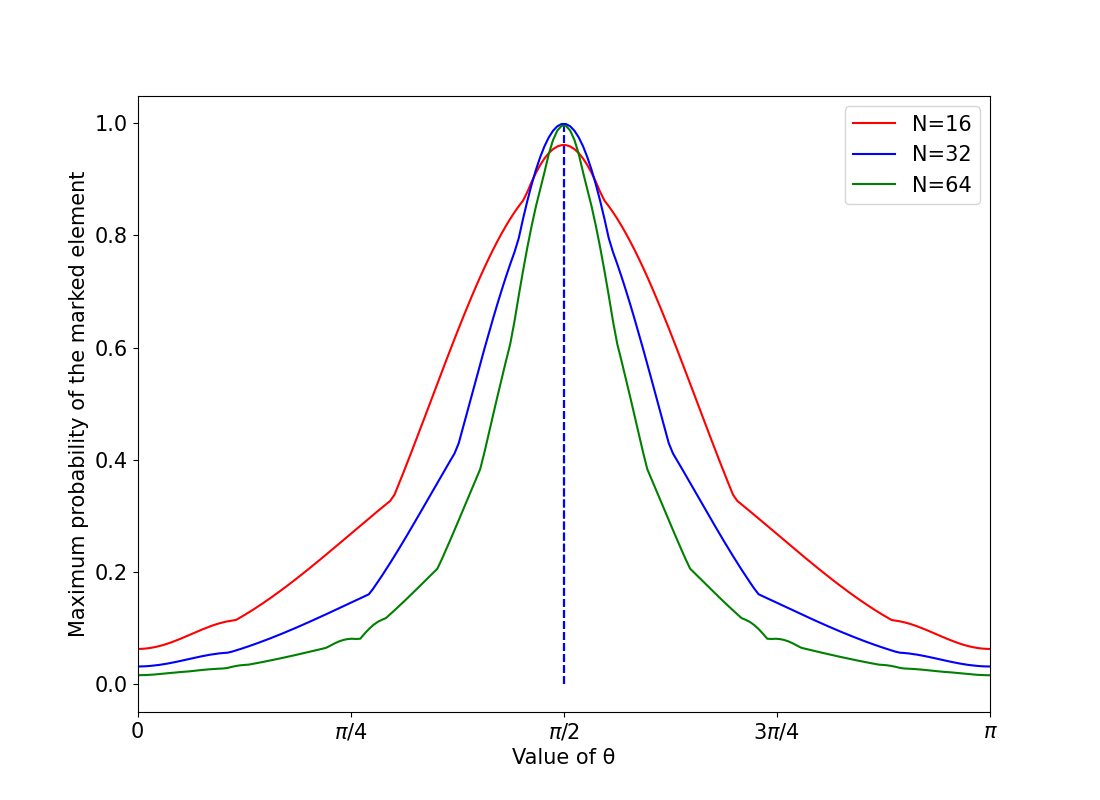
\includegraphics[scale=0.40]{img/StagQuantumWalk/Search/Theta163264.png}
                     \caption{Maximum probability of the marked element as a function of the $\theta$ value plotted from $0$ to $\pi$ for number of nodes $N=64,128$ and $256$.} 
                     \label{fig:stagMultTheta}
              \end{figure}
              Since $H_\alpha^2 = I$, equation \ref{eq:stagQWSearchUnmodEvo1} can be rewritten as
              \begin{equation}
                  U = e^{-i\frac{\pi}{2} H_\alpha} = \cos{\frac{\pi}{2}I} + i\sin{\frac{\pi}{2}H_\alpha} = i H_\alpha = i(2\ket{\alpha_0}\bra{\alpha_0} - I).
              \end{equation}\par
               Having defined the the evolution operator associated with the complete graph, the next step is to use the oracle
                \begin{equation}
                    \mathcal{F'} = I_N - 2\ket{0}\bra{0},
                \end{equation}
                to create the modified evolution operator associated with the search
                \begin{equation}
                    U' = U\mathcal{F'}.
                \end{equation}\par
                The walk achieves the same result as Grover's algorithm after $\frac{\pi}{4}\sqrt{N}$ steps, as shown in figure \ref{fig:StagSearch}. This plot also shows that the probabilities converge to $1$ as $N$ increases, this is because time is discretized and deviations to the ideal steps will matter less for bigger values of $N$.
            	\begin{figure}[!h]
                    \centering
                    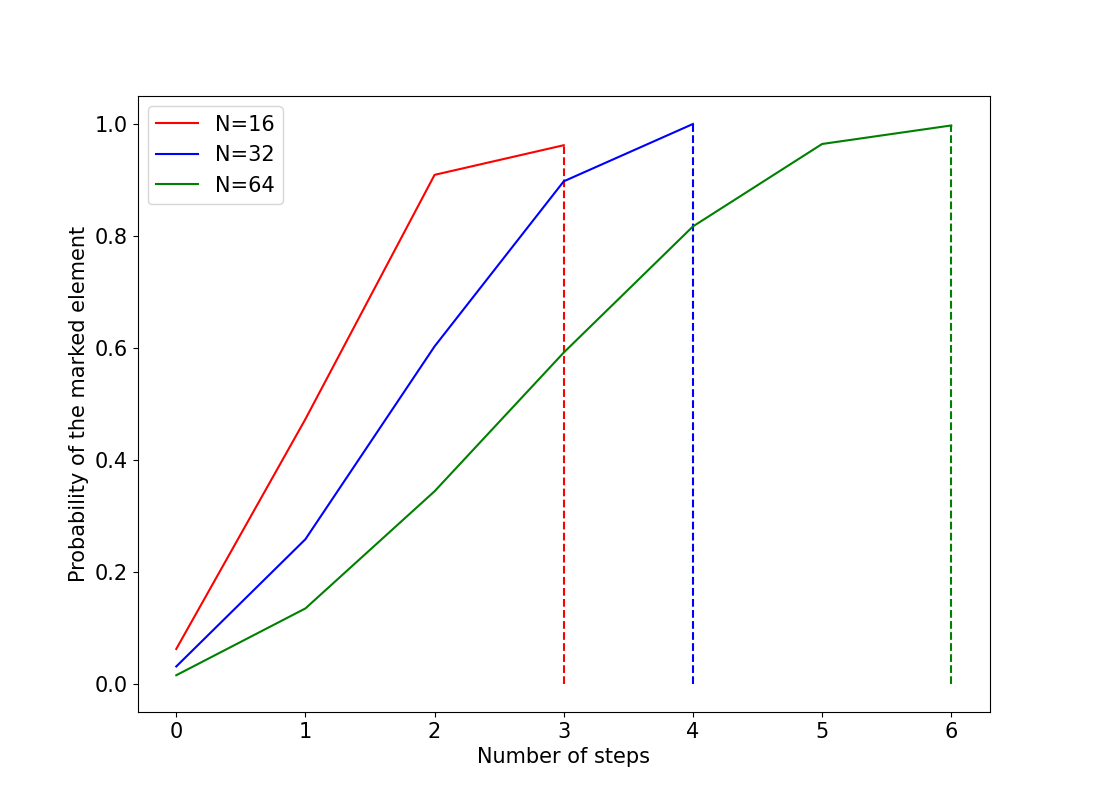
\includegraphics[scale=0.40]{img/StagQuantumWalk/Search/163264.png}
                     \caption{Staggered quantum walk search for a complete graph with 16, 32 and 64 nodes.}\label{fig:StagSearch}
                \end{figure}
                
                %probabilidade em pi/4 sqrt(N)
                %probabilidade mais perto de 1 quanto maior o N, devido à natureza discreta da walk.
               
               \textcolor{red}{precisa de um fechamento também aqui}
                
             \subsection{Continuous}
                As was previously seen, the continuous-time quantum walk model is defined by an evolution operator obtained by solving Schrödinger's equation
                \begin{equation}
                    U(t) = e^{-iHt}.
                \end{equation}
                The search problem requires introducing an oracle to the Hamiltonian, that will mark an arbitrary vertex $m$ %meter que pertence a um conjunto de vertices marcados. chamar vertex onde tenho node.
                \begin{equation}
                    H' = -\gamma L - \ket{m}\bra{m}.
                \end{equation}
                Since the complete graph is a regular graph, the operator can be rewritten in terms of the adjacency matrix plus the marked element. Considering $\ket{0}$ is marked,
                \begin{equation}
                   U'(t) = e^{iH't} = e^{i(-\gamma L - \ket{0}\bra{0})t} = e^{i(-\gamma A + \gamma D - \ket{0}\bra{0})t} = e^{-i\gamma(A+\ket{0}\bra{0})t + i\gamma D t}.
                \end{equation}
                The degree matrix is again $D=dI$, which means it will commute with $A+\ket{0}\bra{0}$ and become a global phase
                \begin{equation}
                U'(t) = e^{-i\gamma(A+\ket{0}\bra{0})t}e^{i\gamma D t} = \phi(t)e^{-i\gamma(A+\ket{0}\bra{0})t}.
                \end{equation}\par
                As was show by \cite{zalka1999}, the value of $\gamma$ is crucial for the success of the search. As $\gamma$ increases, the contribution of the marked element in the Hamiltonian decreases, and as $\gamma$ approaches $0$ the contribution of the adjacency matrix decreases. To find the optimum value, the Hamiltonian can be rewritten by adding multiples of the identity matrix to the adjacency matrix \textcolor{red}{H' é uma notação ruim, confunde com derivada e acredito não ser necessário aqui}
                \begin{equation}
                    H' = -\gamma(A+NI) - \ket{0}\bra{0} = -\gamma N\ket{s}\bra{s} - \ket{0}\bra{0}
                \end{equation}
                where $\ket{s} = \frac{1}{\sqrt{N}}\sum_i \ket{i}$. Now it is obvious that, for $\gamma = \frac{1}{N}$, the Hamiltonian is $H = -\ket{s}\bra{s} - \ket{0}\bra{0}$. It's eigenstates are proportional to $\ket{s}\pm\ket{w}$ and eigenvalues are $-1 - \frac{1}{\sqrt{N}}$ and $-1 + \frac{1}{\sqrt{N}}$, respectively. This means that the evolution rotates from the state of balanced superposition to the marked vertex state in time $\frac{\pi}{\Delta E} = \frac{\pi}{2}\sqrt{N}$ which is, as was shown by \cite{zalka1999}, optimal and equivalent to Grover's algorithm. Plotting $\Delta E$ as a function of $\gamma N$, as can be seen in figure \ref{fig:gamma512}, has a minimum at $\gamma N =1$. The difference between the largest eigenvalue and second largest, plotted in the y-axis, is the smallest for a value of $\gamma N = 1 \implies \gamma =\frac{1}{N}$, which will correspond to the maximum probability for the marked vertex, in optimal steps.
                
                \begin{figure}[h]
                    \centering 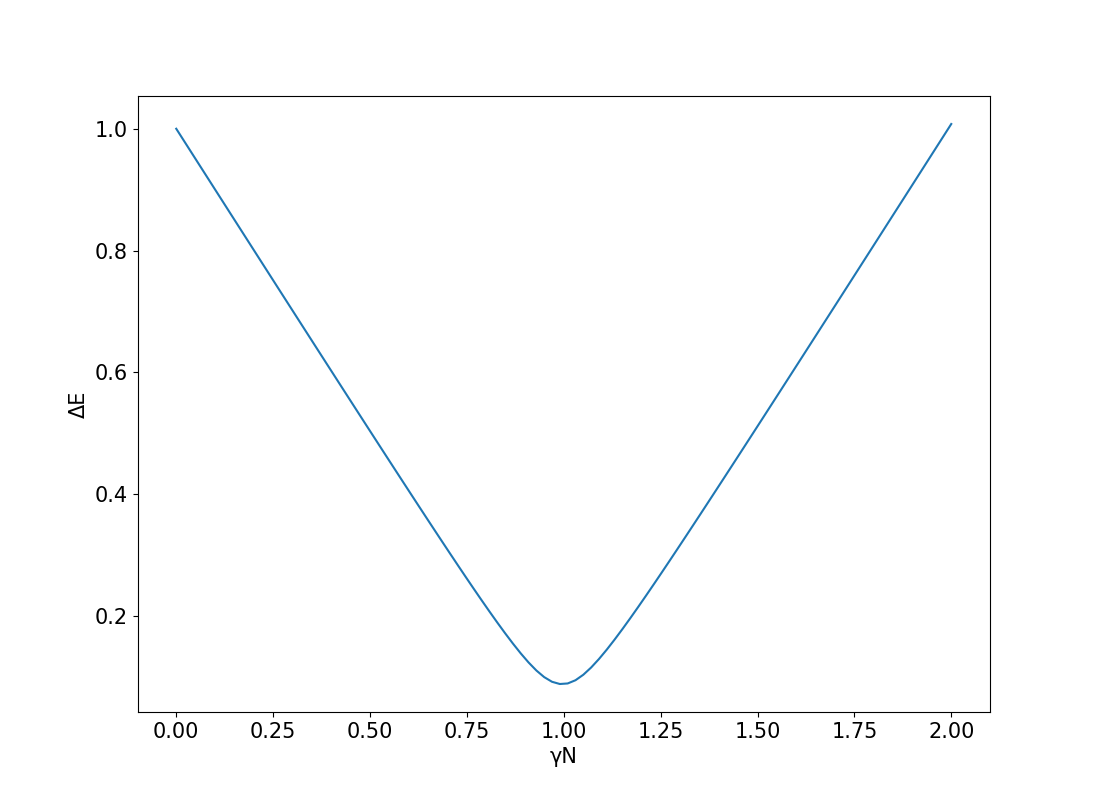
\includegraphics[scale=0.40]{img/ContQuantumWalk/Search/gamma512.png}
                     \caption{Value of the difference between the largest eigenvalue and the second largest, plotted as a function of $\gamma N$, for $N=512$. }\label{fig:ContSearch}
                     \label{fig:gamma512}
                \end{figure}
                
                Figure \ref{fig:ContSearch} shows the evolution of the probability of the marked vertex in time, which is continuous in this model. In contrast with previous models, the distributions are smooth and reach exactly one, since the walk is allowed to evolve to exactly the ideal time steps.
                
                %figura da caminhada com passos ideais
            	\begin{figure}[!t]
                    \centering 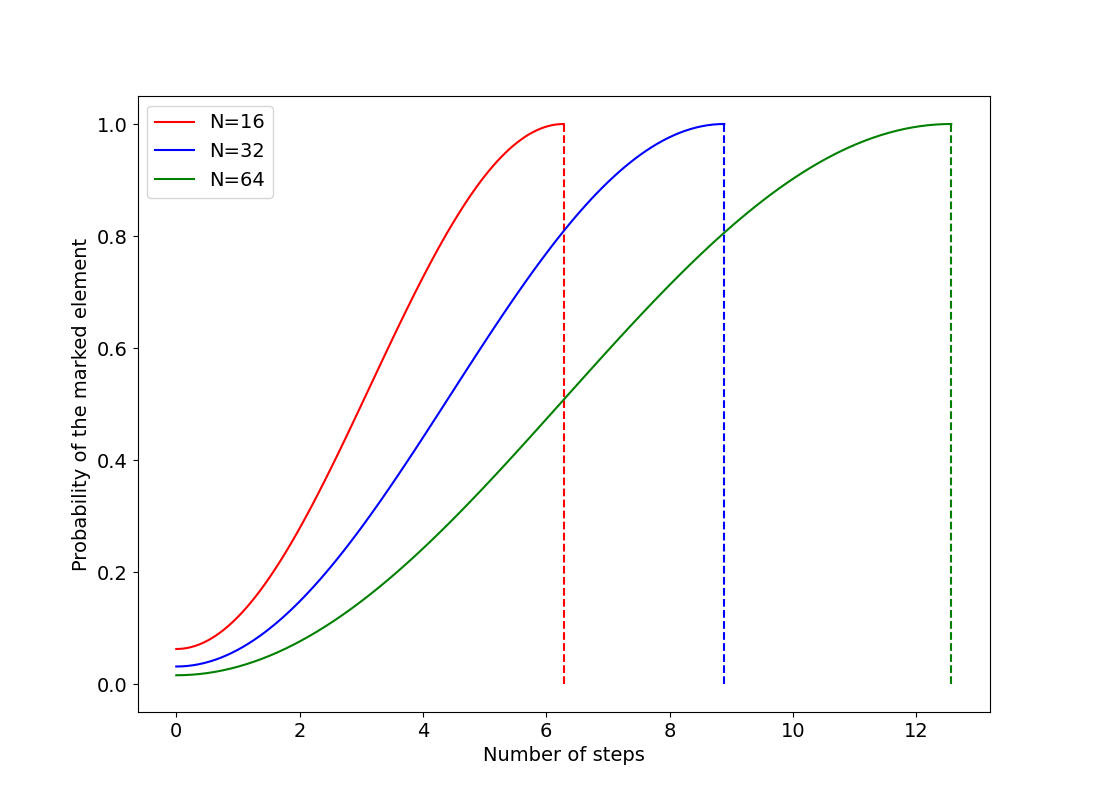
\includegraphics[scale=0.40]{img/ContQuantumWalk/Search/163264.png}
                     \caption{Continuous quantum walk search for a complete graph with 16, 32 and 64 vertices.}\label{fig:ContSearch}
                \end{figure}
                
                %Descrever a figura

